\chapter{The challenge}\label{chap:3}
\epigraph{ Provando e riprovando.}{Accademia del Cimento, Florence, 1675.}
Here we start explaining the actual competition. First of all, what we have to do it is simply simulate an Hamiltonian as explained in chapter~\ref{chap:2}, nothing more. The Hamiltonian will be presented shortly in \ref{sec:xxx}. There are however some restriction:
\begin{enumerate}
    \item Trotterization must be used in the decomposition and the number of steps should be greater or equal to four.
    \item The simulation will be tested and executed on a specific device, Jakarta, that we will describe in \ref{sec:jakarta}
\end{enumerate}

Note that the access to the real device is tied to a long (very long!) queue and time of execution itself is quite long too. That's why IBM provide backend simulators, i.e. classical computer that simulates specifically quantum backends.
Of course we will use \mintinline[breaklines]{python}{sim_noisy_jakarta = QasmSimulator.from_backend(provider.get_backend('ibmq_jakarta'))} which is the simulator of Jakarta on a classical device. Of course simulations are not as near as precise as executions on the real device, however they can guide you towards the right direction, saving execution on the real device for more fine-grained refinements.

There are even backends simulators without noise, however they were not used as, after some testing, they seemed completely out of touch with the results of the real device.
\section{The XXX Model}\label{sec:xxx}

The quantum Heisenberg model, developed by Werner Heisenberg, is a statistical mechanical model used in the study of critical points and phase transitions of magnetic systems, in which the spins of the magnetic systems are treated quantum mechanically. The model is based on the Hamiltonian~\cite{enwiki:1068863987}:
    \begin{equation}
        H = -1/2 \sum_{j=1}^{N} (J_x \sigma_x^{j} \sigma_x^{j+1} + J_y \sigma_y^{j} \sigma_y^{j+1} + J_z \sigma_z^{j} \sigma_z^{j+1})
     \end{equation}

     where $J$ is the coupling constant. We will use a simplified version. This version of the general Heisenberg spin model is called $XXX$ because the same $J$ value multiplies each pair of Pauli operators.




     \begin{equation}
        H_{\text{Heis}} = \sum_{\langle ij \rangle}^{N} J \left(\sigma_x^{(i)}\sigma_x^{(j)} + \sigma_y^{(i)}\sigma_y^{(j)} + \sigma_z^{(i)}\sigma_z^{(j)}\right).
     \end{equation}
    
    
    $N$ is the number of spin-1/2 particles in model.The $i$ and $j$ superscripts label which qubit they act on. For example, $\sigma_x^{(1)}$ would be the $\sigma_x$ operator acting on only qubit 1 (which is the 2nd qubit since indexing starts at 0). The sum notation $\langle ij \rangle$ means the sum is over nearest neighbors (only qubits next to each other interact), and $J$ is the interaction strength, which we will set $J=1$.

    

    Of course $\sigma_x, \sigma_y, \sigma_z$ are the known pauli matrices: 

\[
    \sigma_x =
    \begin{pmatrix}0&1\\1&0\end{pmatrix}
    \]
    \[
    \sigma_y =
    \begin{pmatrix}0&-i\\i&0\end{pmatrix} 
    \]
    \[
    \sigma_z =
    \begin{pmatrix}1&0\\0&-1\end{pmatrix} 
    \]


    We will work with the explicit case of $N=3$ with the 3 spins arranged in a line. Written out fully, the Hamiltonian is
\begin{equation}
\begin{split}
H_{\text{Heis3}} &= \sigma_x^{(0)}\sigma_x^{(1)} + \sigma_x^{(1)}\sigma_x^{(2)} + \sigma_y^{(0)}\sigma_y^{(1)} \\
&+ \sigma_y^{(1)}\sigma_y^{(2)} + \sigma_z^{(0)}\sigma_z^{(1)} + \sigma_z^{(1)}\sigma_z^{(2)}.
\end{split}
\end{equation}
Now that we have a Hamiltonian ($H_{\text{Heis3}}$), we can use it to determine how the quantum system of 3 spin-1/2 particles changes in time.


To compute the matrix representation of $H_{\text{Heis3}}$, we are actually missing some pieces namely the identity operator $I$ and the tensor product $\otimes$ symbol. They are both often left out in when writing a Hamiltonian, but they are implied to be there. 

Writing out the full $H_{\text{Heis3}}$ including the identity operators and tensor product symbols we obtain: 

\begin{equation}
    \begin{split}
H_{\text{Heis3}} &= \sigma_x^{(0)}\otimes\sigma_x^{(1)}\otimes I^{(2)} + I^{(0)} \otimes\sigma_x^{(1)}\otimes\sigma_x^{(2)} \\ &+ \sigma_y^{(0)}\otimes\sigma_y^{(1)}\otimes I^{(2)} + 
I^{(0)} \otimes \sigma_y^{(1)}\otimes\sigma_y^{(2)} \\ &+ I^{(0)} \otimes\sigma_z^{(0)}\otimes\sigma_z^{(1)} + I^{(0)}\otimes\sigma_z^{(1)}\otimes\sigma_z^{(2)}.
\end{split}
\end{equation}


Knowing the Hamiltonian, we can determine how quantum states of that system evolve in time by solving the Schrödinger equations
\begin{equation}
i\hbar \dfrac{d}{dt}|\psi(t)\rangle = H |\psi(t)\rangle
\end{equation}

For simplicity, let's set $\hbar = 1$. We know that the Hamiltonian $H_{\text{heis3}}$ does not change in time, so the solution to the Schrödinger equation is an exponential of the Hamiltonian operator

\begin{align}
U_{\text{Heis3}}(t) &= e^{-it H_\text{Heis3}} = \exp\left(-it H_\text{Heis3}\right) \\
U_{\text{Heis3}}(t) &= \exp\left[-it \sum_{\langle ij \rangle}^{N=3} \left(\sigma_x^{(i)}\sigma_x^{(j)} + \sigma_y^{(i)}\sigma_y^{(j)} + \sigma_z^{(i)}\sigma_z^{(j)}\right) \right]
\end{align}



\begin{equation}
    \begin{split}
        U_{\text{Heis3}}(t) &= \exp\left[-it \left(\sigma_x^{(0)}\sigma_x^{(1)} + \sigma_x^{(1)}\sigma_x^{(2)} + \sigma_y^{(0)}\sigma_y^{(1)}  + \sigma_y^{(1)}\sigma_y^{(2)} + \sigma_z^{(0)}\sigma_z^{(1)} + \sigma_z^{(1)}\sigma_z^{(2)}\right) \right]
    \end{split}
\end{equation}
Now that we have the time evolution operator $U_{\text{Heis3}}(t)$, we can simulate changes in a state of the system ($|\psi(t)\rangle$) over time $|\psi(t)\rangle = U_{\text{Heis3}}(t)|\psi(t=0)\rangle$. 

Our goal will be to decompose $U_{\text{Heis3}}(t)$ into one and two-qubit gates executable in the Jakarta device.
\section{Quantum bits}
The definition of qubit (quantum bit) immediately follows from \hyperref[postulate:1]{postulate 1}:
\begin{defn}
A \emph{qubit} is a physical system $Q$ whose Hilbert space $\mathcal{H}_Q$ has dimension $\dim\mathcal{H}_Q = 2$.
\end{defn}
Because of \hyperref[postulate:1]{postulate 1} and according to the definition of vector space we see that every linear combination of a state vector
\begin{equation}\label{eq:linear-combination}
  \ket{\psi} = a \ket{\alpha} + b \ket{\beta} \quad \ket{\alpha},\ket{\beta} \in \mathcal{H}_\psi \quad a,b \in \mathbb{C} \quad \abs*{a}^2 + \abs*{b}^2 = 1
\end{equation}
is still part of the state space and it still describes the physics of the system. (There is only a constraint: the state has to be normalized according to \eqref{eq:normalization}, such a rescaling is possible and will be assumed hereafter.) 


Here lies the main difference between bits and qubits: whereas in classical computation only $0$ and $1$ states are allowed, in quantum computation also superposition states are perfectly acceptable.\graffito{Main difference between bits and qubits.} 
What does a superposition state physically mean? If we measure for example \eqref{eq:linear-combination} the probability of being in the state $\ket{\alpha}$ is  $\abs*{a}^2$ and the probability of being in the state $\ket{\beta}$ is $\abs*{b}^2$.

According (again) to the \hyperref[postulate:1]{first postulate} the state of a qubit is a vector in a two-dimensional Hilbert space. Let us define its basis:
\begin{defn}\label{def:computational-basis}
The orthonormal basis of the two-dimensional Hilbert space describing a qubit is called \emph{computational basis} and it's composed of the states $\ket{0}$ and $\ket{1}$ known as \emph{computational basis states}.
\end{defn}
How a qubit is physically made?
It can be a $1/2$ spin particle, an atomic system whose dynamics is described by two (non-degenerate) energy levels and so on.
Whatever we choose to be our physical realization of the qubit we have a Hermitian operator associated with the observable chosen. The computational basis then will be composed by the eigenstates of the Hermitian operator associated with the observable\footnote{To every Hermitian operator $\Omega$ defined on a space $\mathcal{H}$ there exist (at least) a basis of the space $\mathcal{H}$ consisting of the orthonormal eigenvectors of the operator \cite[36]{Shankar}.}, those state (whatever the operator is) will be labelled as $\{\ket{0},\ket{1}\}$ according to \hyperref[def:computational-basis]{definition 2}.


Let us use, for example, a $1/2$ spin particle.   We know that the Hermitian operator associated with spin is $S_z$ or $\hat{\sigma}_z = \frac{2}{\hbar} S_z$ that fits our scope because it has two eigenstates and two non-degenerate eigenvalues: 
\graffito{An example of how a qubit can be physically implemented.}

\begin{equation}\label{eq:spin-particle}
\begin{split}
    \hat{\sigma}_z \ket{\chi_+} &= \ket{\chi_+}  \\
    \hat{\sigma}_z \ket{\chi_-} &= -\ket{\chi_-}\,.
\end{split}
\end{equation}
These eigenstates (i.e. the spinors) span a two-dimensional Hilbert space and can be chosen as the computational basis.

\subsection{Quantum register}
The definition of quantum register, quantum analogue of the classical register, immediately follows from \hyperref[postulate:4]{postulate 4}:
\begin{defn}
A $n$ size \emph{quantum register} is a system QR with $\dim\mathcal{H}_{QR} = 2^n$.
\end{defn}
In other words, a quantum register is a system comprising multiple qubits.


The simplest case is a system $N=2$ with two qubits $Q_1$ and $Q_2$. If we define the basis of $\mathcal{H}_{Q_1}$ and $\mathcal{H}_{Q_2}$ as $\{\ket{0}_1, \ket{1}_1\}$ and $\{\ket{0}_2, \ket{1}_2\}$ one possible basis of $H_{QR}$ is \graffito{Quantum register with two qubits.}
\begin{equation}\label{eq:quantum-register-basis}
    \{\ket{0}_1 \otimes \ket{0}_2, \ket{1}_1 \otimes \ket{0}_2, \ket{0}_1 \otimes \ket{1}_2, \ket{1}_1 \otimes \ket{1}_2\}\
\end{equation}
and as expected we have $\dim\mathcal{H}_{QR} = 4$.
\subsection{Entanglement}
Consider two arbitrary quantum systems $Q_1$ and $Q_2$, with respective Hilbert spaces $\mathcal{H}_{Q_1}$ and $\mathcal{H}_{Q_2}.$ The Hilbert space of the composite system is the tensor product: 
\begin{equation*}
\mathcal{H}_{Q_1} \otimes \mathcal{H}_{Q_2}\,,
\end{equation*}
if the first system is in state $\ket{\psi}_{Q_1}$ and the second in state $\ket{\psi}_{Q_2}$ the state of the composite system is
\begin{equation*}
    \ket{\psi}_{Q_1} \otimes \ket{\psi}_{Q_2}\,.
\end{equation*}
States of the composite system that can be represented in this form are called \emph{separable states} while
\begin{defn}
A composite system such that $\ket{QR} \neq \otimes_i \ket{Q_i}$ is an \emph{entangled state}.
\end{defn}

If we consider two qubits:
\graffito{An example of a separable state.}
\begin{align*}
    &\ket{Q_1} = a \ket{0}_1 + b \ket{1}_1 \quad a, b \in \mathbb{C}, \quad \abs*{a}^2 + \abs*{b}^2 = 1 \\
    &\ket{Q_2} = c\ket{0}_2 + d\ket{1}_2 \quad c,d \in \mathbb{C}, \quad \abs*{c}^2 + \abs*{d}^2 = 1
\end{align*}
the overall state of the system is:
\begin{multline*}
    \ket{QR} = \ket{Q_1} \otimes \ket{Q_2} = ac \ket{0}_1 \otimes \ket{0}_2 \\ +  bc  \ket{1}_1 \otimes \ket{0}_2 + 
    ad \ket{0}_1 \otimes \ket{1}_2 + bd \ket{1}_1 \otimes \ket{1}_2
\end{multline*}
that is a separable state.

If instead we have:
\graffito{An example of an entangled state.}
\begin{equation*}
    \ket{\Phi^+} = \frac{\ket{0}_1 \otimes \ket{0}_2 + \ket{1}_1 \otimes \ket{1}_2}{\sqrt{2}}
\end{equation*}
we immediately see that this is an entangled state\footnote{It is one of the Bell states, four specific maximally entangled quantum states of two qubits.} as there is no way of writing it as $\ket{Q_1} \otimes \ket{Q_2}$. 
\section{Jakarta}\label{sec:jakarta}
Jakarta is a 7-qubit machine, with a Falcon r5.11H processor. 

Why 7 qubit is our Hamiltonian has only tree states? 
The other four states can be used as ancilla qubits in the decomposition and/or to reduce noise in noise reduction techniques. State Tomography at the end will be done only on qubit 1,3,5 (and you can't change which qubits will me measured) while other qubits will not be measured and so they are free to use as one like.

\paragraph{Gates}
We can use the native gates of the machine, the following set of gates are universal, therefore any gate can be implemented even without Qiskit Pulse, however there could be a significant improvement using only native gates\footnote{e.g. avoiding overlapping of errors of the native gates}. Here is the list:
   \begin{description}
    \item[\textbf{ID}: ] Identity
    \item[\textbf{CNOT}: ] CNOT Gate
    \item[\textbf{Z}: ] Z Gate
    \item[\textbf{SX}: ] Pauli-X Gate Squared
    \item[\textbf{X}: ] Pauli-X Gate
   \end{description}

In figure~\ref{fig:jakarta1} and figure~\ref{fig:jakarta2} we see the full specifications of Jakarta. Specifically in figure~\ref{fig:jakarta2} we see the various errors in the native gates. Note that those errors fluctuate quite significantly over time.

In figure~\ref{fig:cnot-error}, figure~\ref{fig:pauli-error} and figure~\ref{fig:sx-error} we see the different errors in the native gates divided per qubit. 

Initially it was attempted to exploit those different errors in order to create a decomposition that uses as less as possibile gates on qubit with high errors on those gates. However, over time, this strategy has not proved to be successful, especially for the already mentioned high fluctuation of errors during time.
    
\begin{figure}
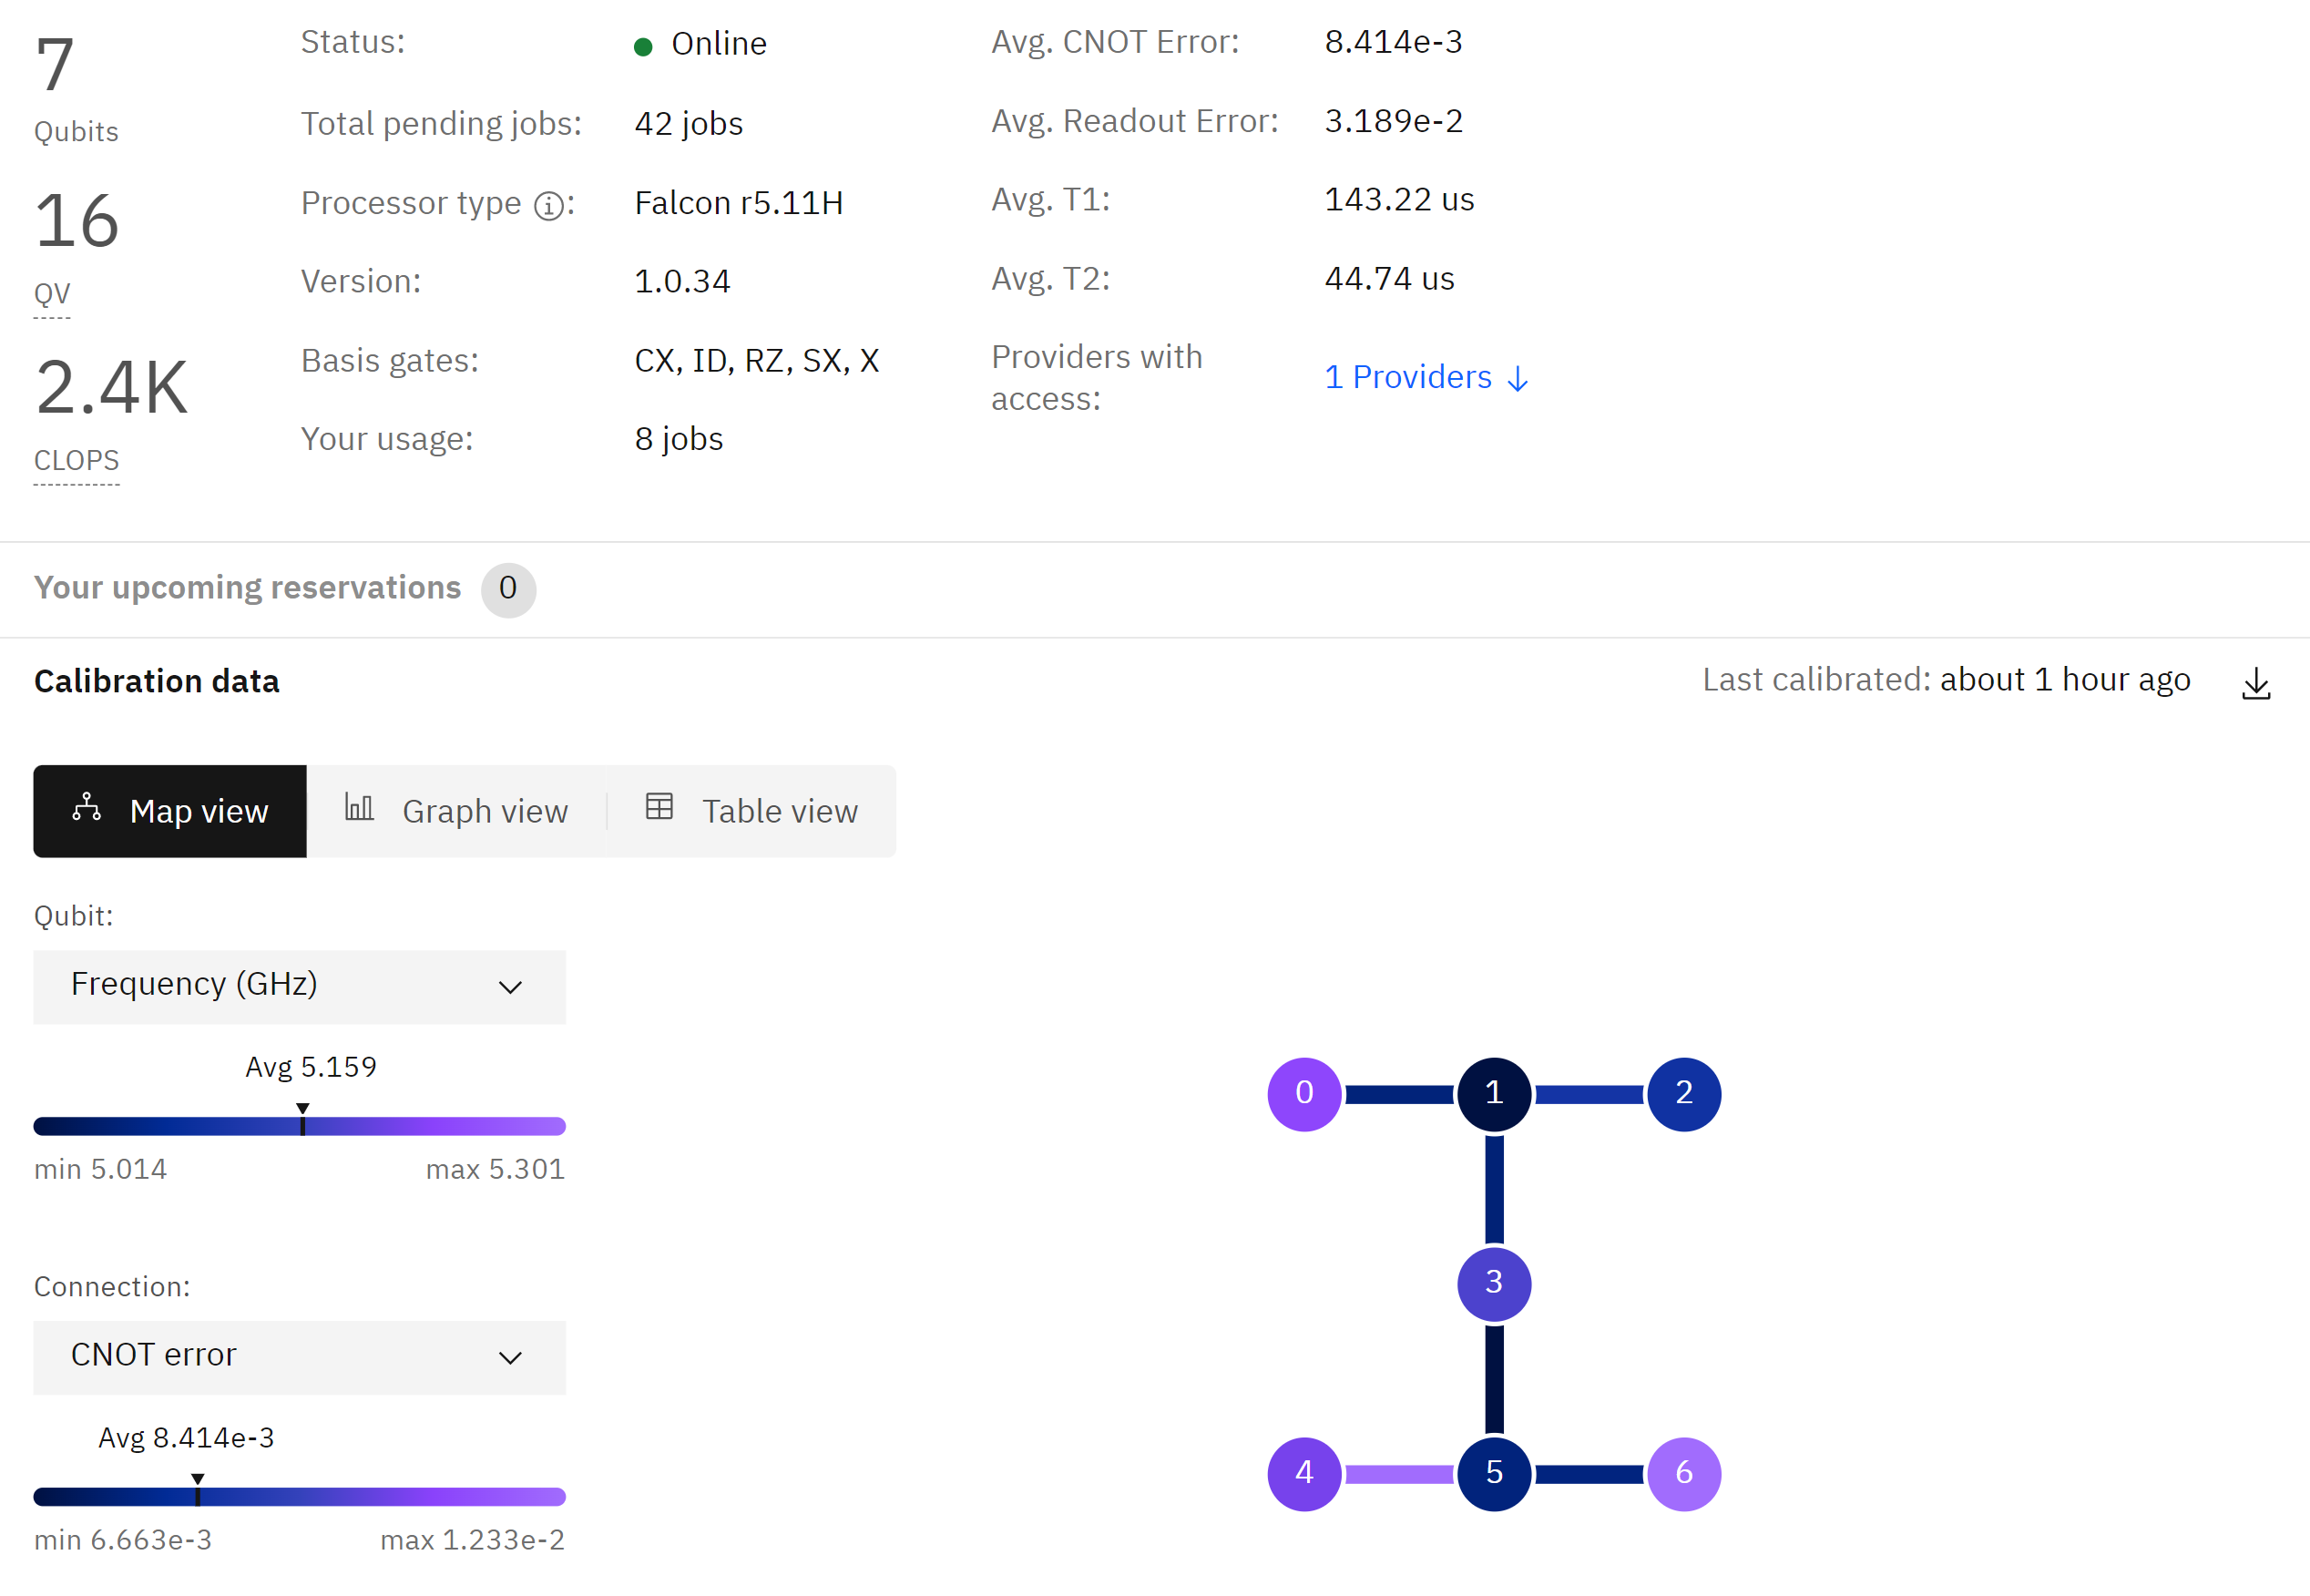
\includegraphics[width = 1.5\textwidth]{jakarta1.png}
\centering
\caption{The machine}
\label{fig:jakarta1}
\end{figure}

\begin{figure}
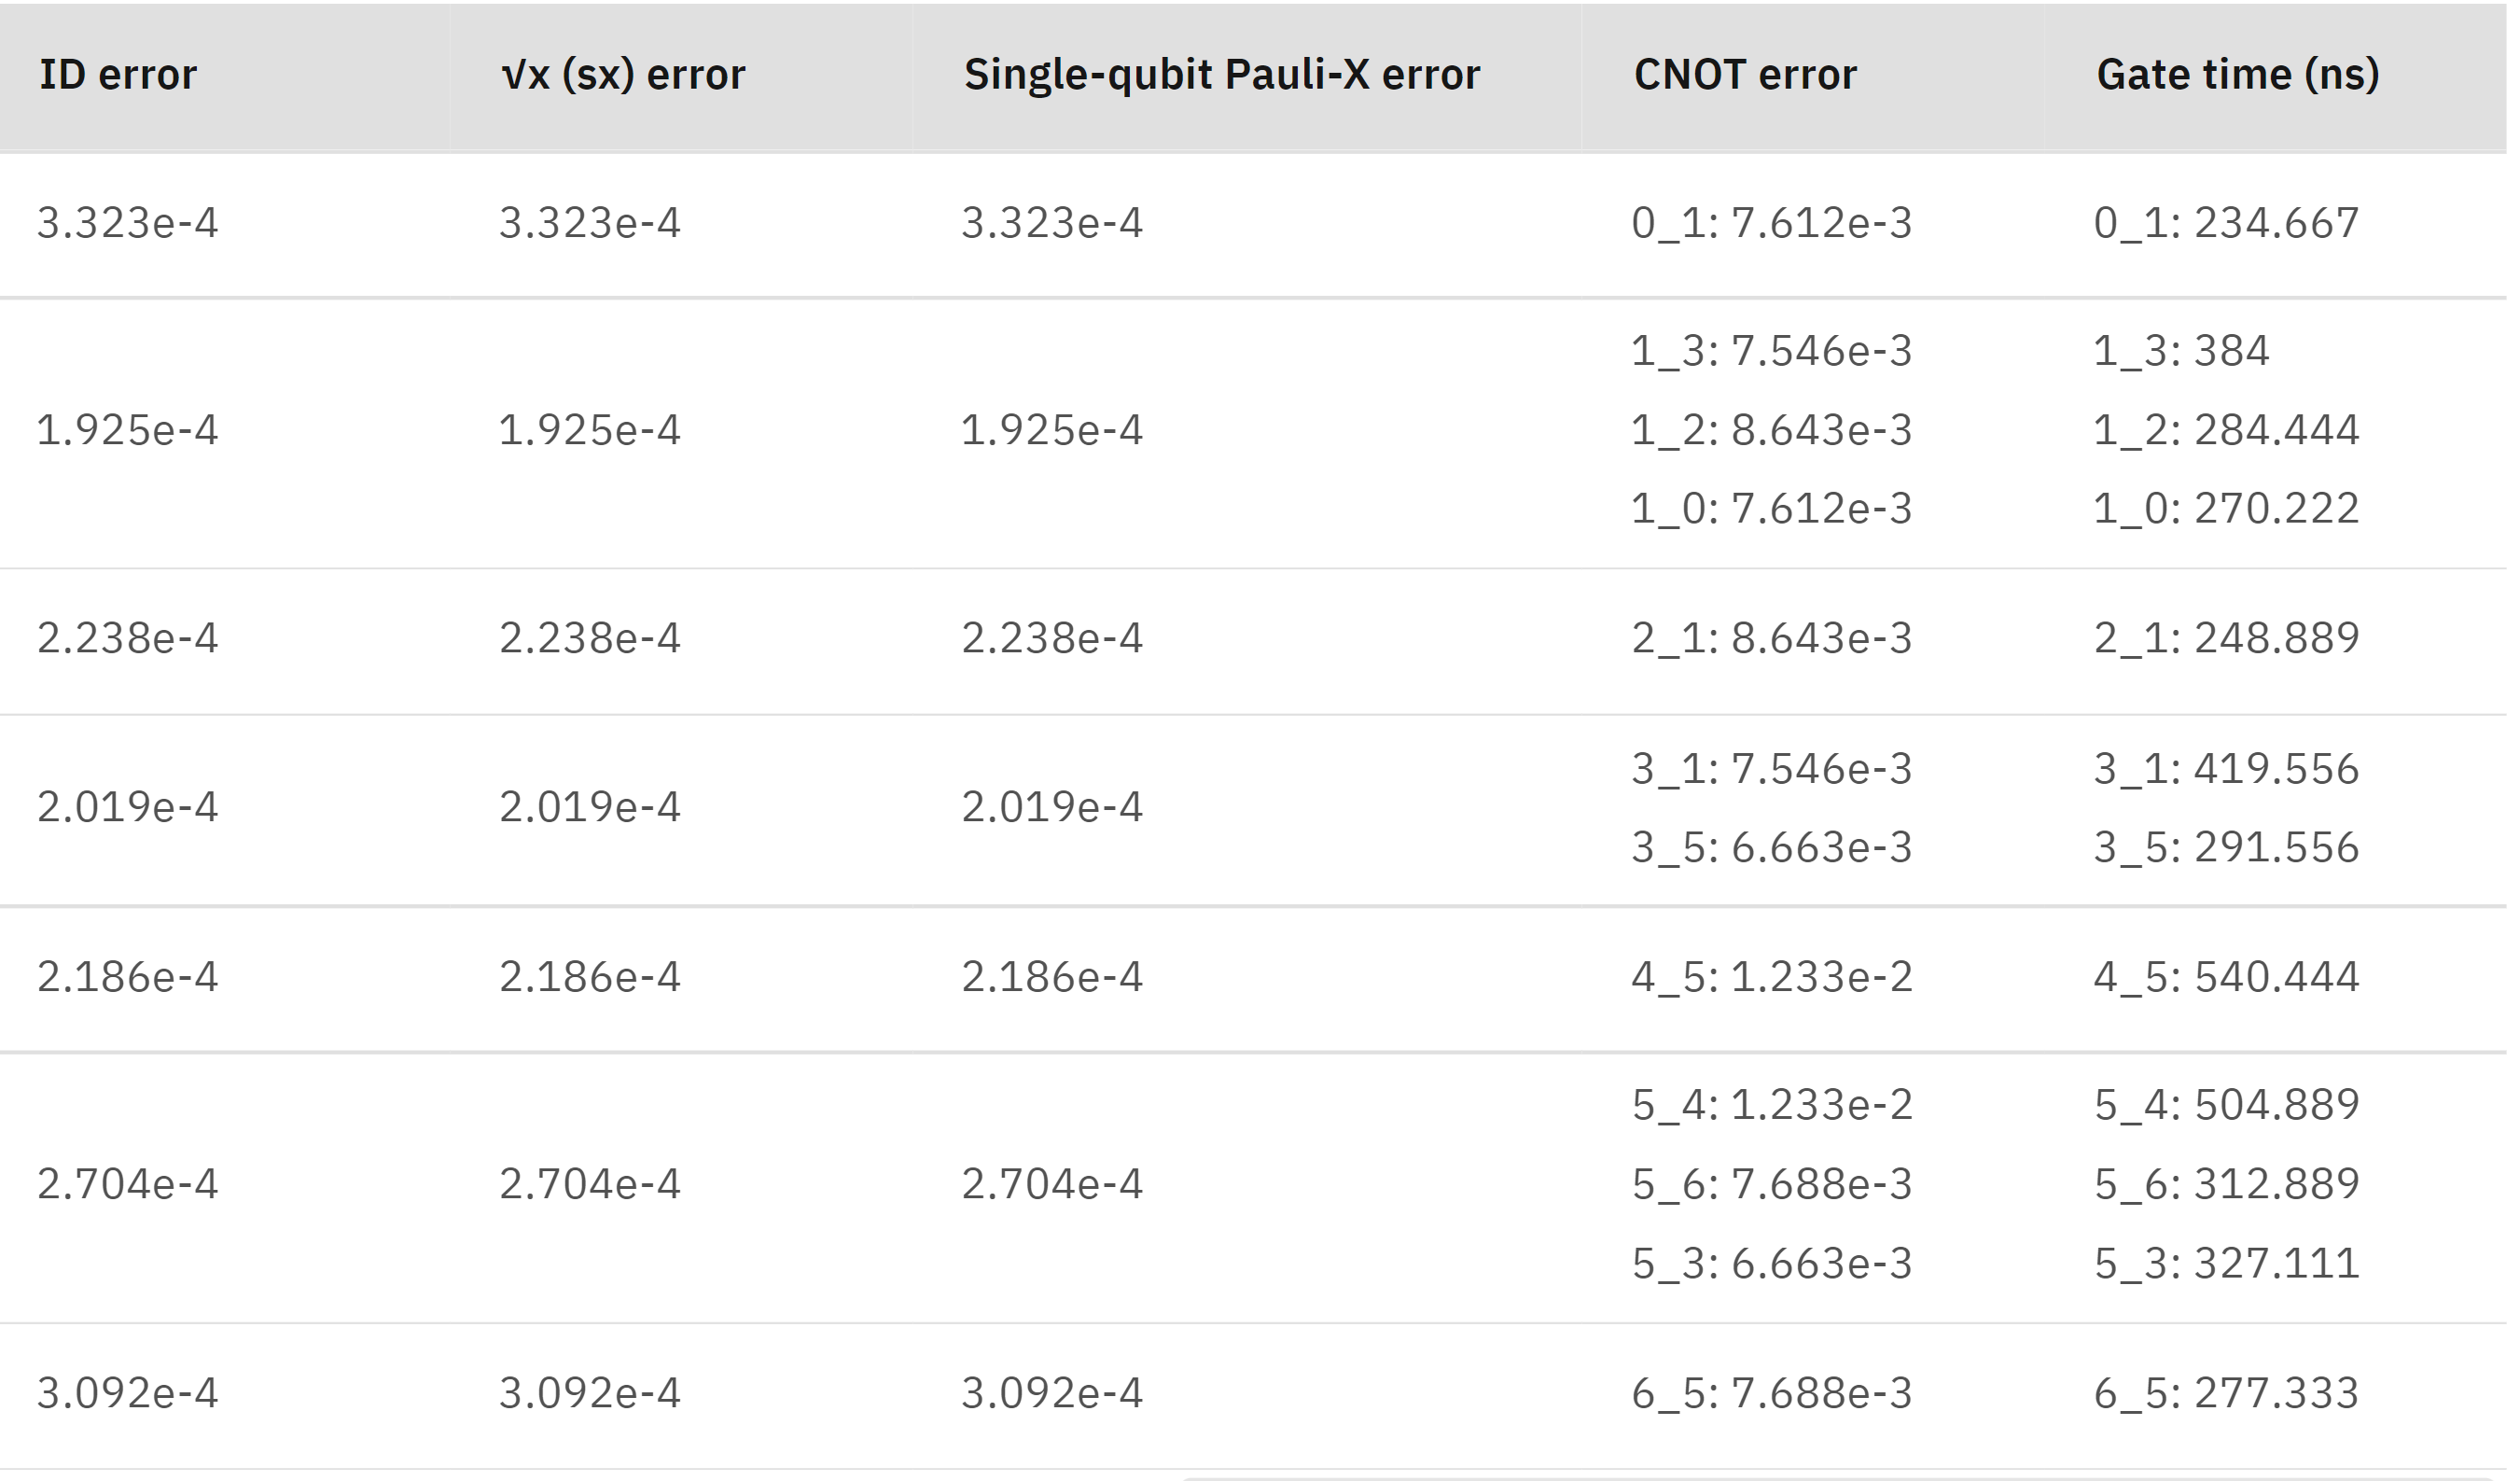
\includegraphics[width = 1.3\textwidth]{jakarta2.png}
\centering
\caption{Gates and errors}
\label{fig:jakarta2}
\end{figure}


\begin{figure}
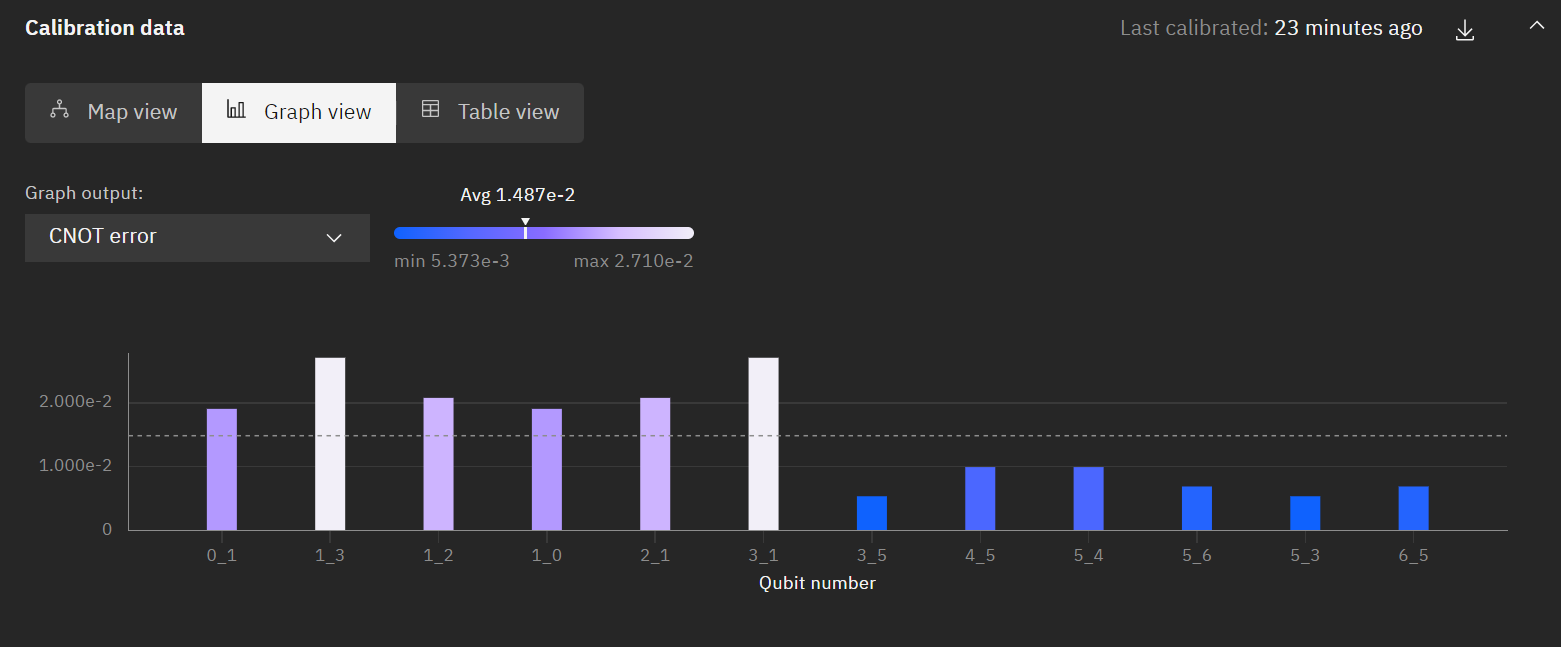
\includegraphics[width = 1.1\textwidth]{error1.png}
\centering
\caption{CNOT errors}
\label{fig:cnot-error}
\end{figure}


\begin{figure}
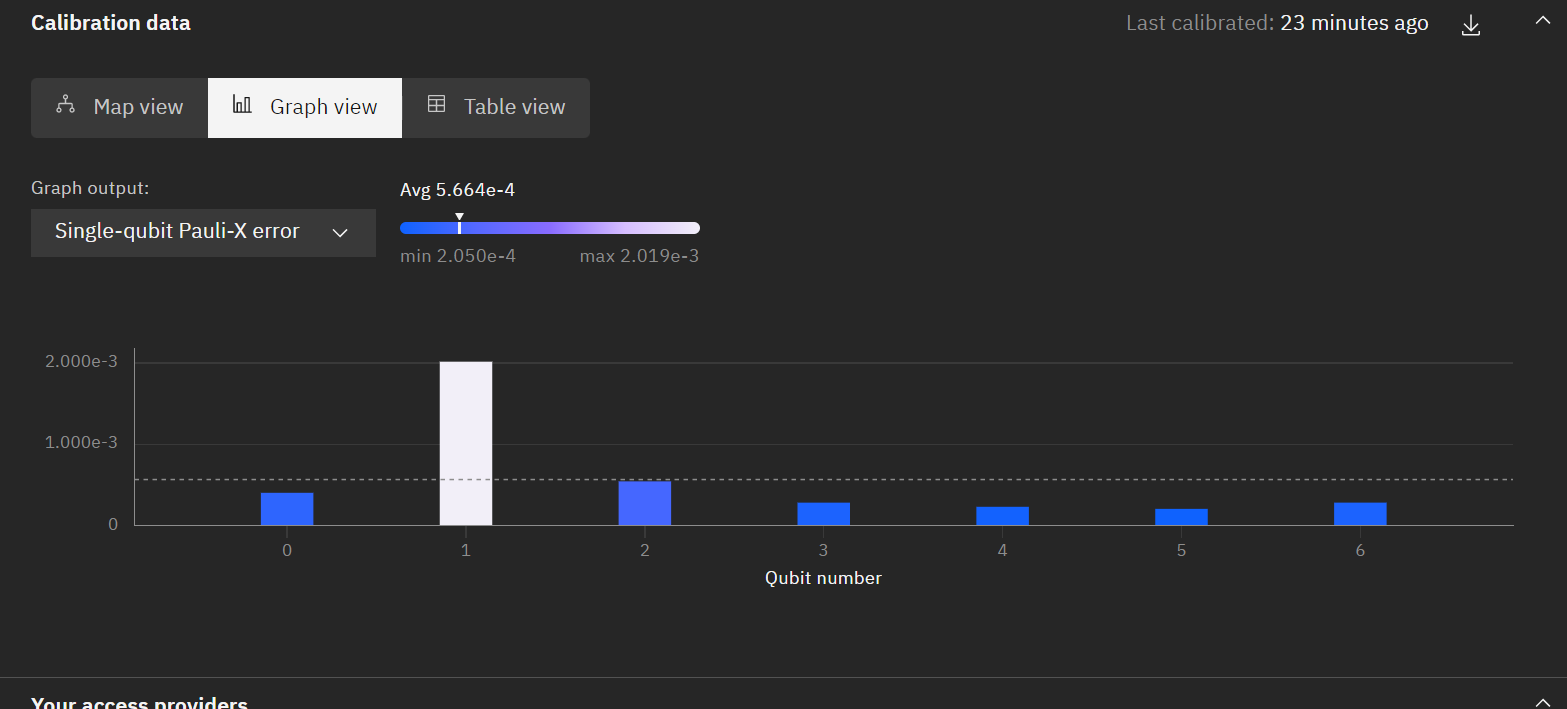
\includegraphics[width = 1.1\textwidth]{error2.png}
\centering
\caption{Single-qubit Pauli-X errors}
\label{fig:pauli-error}
\end{figure}

\begin{figure}
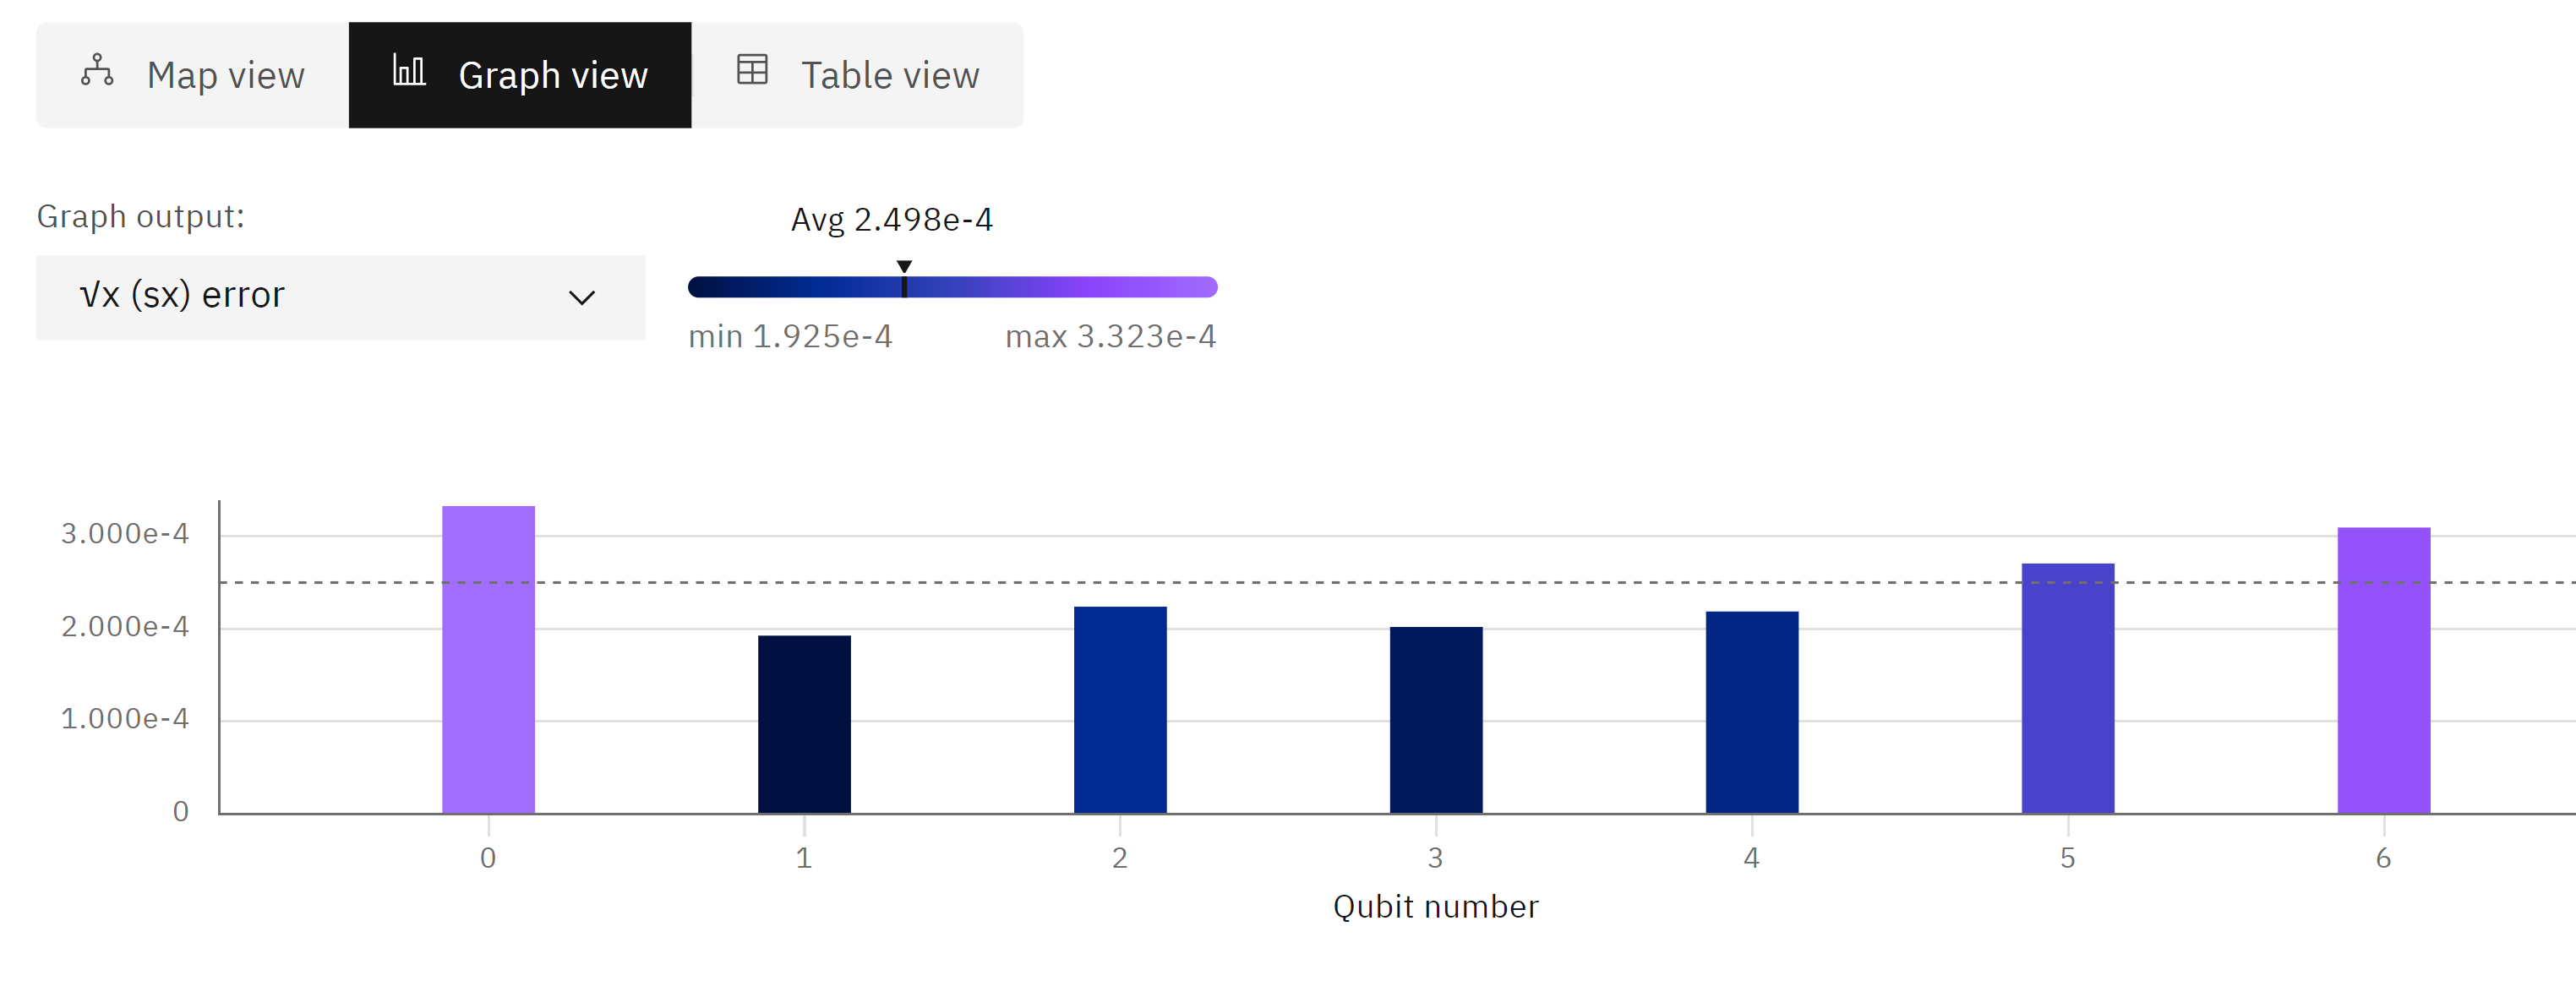
\includegraphics[width = 1.1\textwidth]{error3.png}
\centering
\caption{Sx errors}
\label{fig:sx-error}
\end{figure}

\section{The solution}
We want to decompose 
\begin{equation}
    U_{\text{Heis3}}(t) = \exp\left[-it \sum_{\langle ij \rangle}^{N=3} \left(\sigma_x^{(i)}\sigma_x^{(j)} + \sigma_y^{(i)}\sigma_y^{(j)} + \sigma_z^{(i)}\sigma_z^{(j)}\right) \right]
    \end{equation}
into single and two-qubit gates.

Since the Pauli operators do not commute with each other~\cite{Shankar} the exponential $U_{\text{Heis3}}(t)$ cannot be split into a product of simpler exponentials.

However, we can approximate $U_{\text{Heis3}}(t)$ as a product of simpler exponentials through Trotterization. Consider a subsystem of 2 spin-1/2 particles within the larger 3 spin system. The Hamiltonian on spins $i$ and $j$ ($i,j \in \{0,1,2\}$) would be $H^{(i,j)}_{\text{Heis2}} = \sigma_x^{(i)}\sigma_x^{(j)} + \sigma_y^{(i)}\sigma_y^{(j)} + \sigma_z^{(i)}\sigma_z^{(j)}$. Rewriting $U_{\text{Heis3}}(t)$ in terms of the two possible subsystems within the total $N=3$ system you will simulate,

\begin{equation}
U_{\text{Heis3}}(t) = \exp\left[-i t \left(H^{(0,1)}_{\text{Heis2}} + H^{(1,2)}_{\text{Heis2}} \right)\right].
\end{equation}

$H^{(0,1)}_{\text{Heis2}}$ and $H^{(1,2)}_{\text{Heis2}}$ do not commute, so
\begin{equation}
 U_{\text{Heis3}}(t) \neq \exp\left(-i t H^{(0,1)}_{\text{Heis2}}\right) \exp\left(-i t H^{(1,2)}_{\text{Heis2}} \right)
\end{equation}. 
 
 But, this product decomposition can be approximated with Trotterization which says $U_{\text{Heis3}}(t)$ is approximately a short evolution of $H^{(0,1)}_{\text{Heis2}}$ (time = $t/n$) and followed by a short evolution of $H^{(1,2)}_{\text{Heis2}}$ (time = $t/n$) repeated $n$ times


\begin{align}
U_{\text{Heis3}}(t) &= \exp\left[-i t \left(H^{(0,1)}_{\text{Heis2}} + H^{(1,2)}_{\text{Heis2}} \right)\right] \\
U_{\text{Heis3}}(t) &\approx \left[\exp\left(\dfrac{-it}{n}H^{(0,1)}_{\text{Heis2}}\right) \exp\left(\dfrac{-it}{n}H^{(1,2)}_{\text{Heis2}} \right)\right]^n.
\end{align}


$n$ is the number of Trotter steps, and as $n$ increases, the approximation should becomes more accurate but as we have already anticipated experimentally this not seems to be the case.

But now we have a state of the art solution for decomposing \text{Heis2} into quantum gates~\cite{s1} \cite{s2} and this is shown in figure~\ref{fig:solution}, we can then implement this decomposition of \text{Heis2} into our decomposition of \text{Heis3}.

In the decomposition of Heis2 we have:

\begin{equation}
    R X(\theta)=\exp \left(-i \frac{\theta}{2} X\right)=\left(\begin{array}{cc}
        \cos \frac{\theta}{2} & -i \sin \frac{\theta}{2} \\
        -i \sin \frac{\theta}{2} & \cos \frac{\theta}{2}
        \end{array}\right)
\end{equation}

and 
\begin{equation}
    R Z(\lambda)=\exp \left(-i \frac{\lambda}{2} Z\right)=\left(\begin{array}{cc}
        e^{-i \frac{\lambda}{2}} & 0 \\
        0 & e^{i \frac{\lambda}{2}}
        \end{array}\right).
\end{equation}

Those are not native gates but as already said they can be implemented as Jakarta has a universal set of quantum gates, and we can change the phase factor directly without the need of using Pulse.
\begin{figure}[htb]
    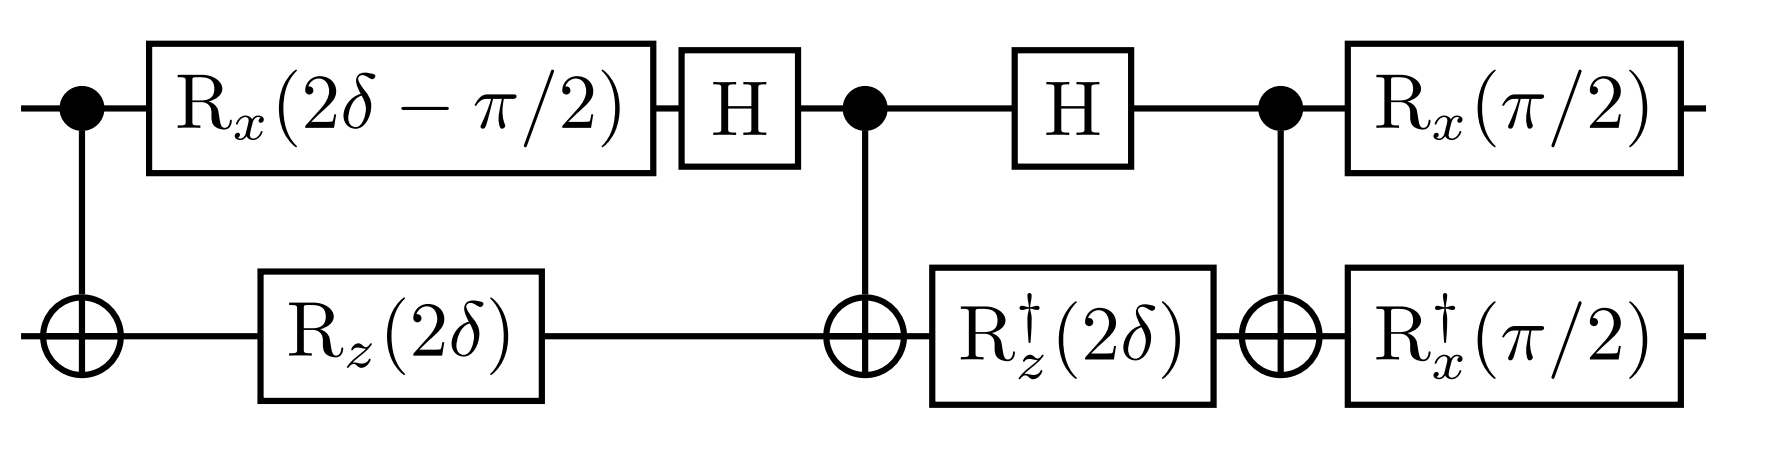
\includegraphics[width = 1.2\textwidth]{circuit.png}
    \centering
    \caption{Heis2 decomposition}
    \label{fig:solution}
\end{figure}


At the end our circuit is represented in figure~\ref{fig:circuit} where we can see the 7 qubits, the 4 trotterization steps and the measure at the end. The circuit of~\ref{fig:solution} is contained in each trotterization step. 
\begin{figure}[htb]
    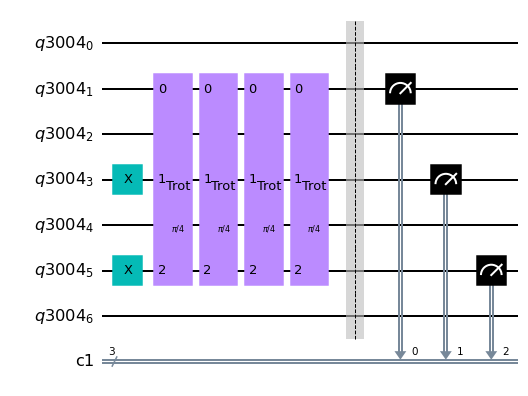
\includegraphics[width = \textwidth]{output1.png}
    \centering
    \caption{Circuit overview}
    \label{fig:circuit}
\end{figure}

Finally, those are the results:
\begin{description}
    \item[Noisy simulation: ]0.4405 ± 0.0011 (N=4)
    \item[Real device: ]0.3108 ± 0.0034 (N=4)
    \end{description}

    You may ask why there were not tried more complicated decomposition, the reason is that at the end reducing the original Hamiltonian to Hamiltonians with already recognized state of the art decomposition resulted to be the strategy that provided the better results, as completely raw decomposition directly to gates resulted in significantly weaker results.

    In addition to that the least number of trotterization steps as the problem required were used. This is because, contrary to what Lie's formula presented in chapter~\ref{chap:2} seems to suggests, experimentally it was very clear that augmenting trotterization steps significantly reduced state tomography results, probably because no noise suppression techniques were used in order to deal with the the fact that the circuit increases with more Trotterization steps.

